% --- Polarisation and choice of contrasts ----------------------------------

\section{Treatment of reference alleles}
\label{sec:reference_alleles}

In the model above we have set the effect of a given allele
(either the reference, major, or ancestral allele) to zero,
and assigned the effect of each other allele an independent Gaussian effect.
This, however, apparently depends on the choice of reference allele,
and so another choice would have been
to assign a separate independent Gaussian effect to \emph{every} allele.
It turns out that this is only equivalent in the biallelic case,
in the sense that there exists a transformation of parameters for one model
that produces the other model.
The situation is essentially that of choosing the contrasts for a factor
when fitting a linear model with Gaussian priors on the parameters:
the BLUPs are the same, but the posterior distributions on the parameters may not be,
because different choices of contrasts include non-equivalent priors.
We have made the allele-symmetric choice
because it is insensitive to the choice of reference allele
and because it fits more naturally in existing schemes for computing with tree sequences.

To see this, consider the (contrived) case in which we have $n$ haploid samples
genotyped at a single locus, and every sample has a distinct genotype.
If we write $Z_k$ as the effect of genotype $k$,
and $Y$ for an intercept,
then $X_k$, the trait value of sample $k$ is 
\begin{align*}
    X_k &= Y + Z_k \\
        &= Y + Z_0 + (Z_k - Z_0) .
\end{align*}
Now, the two models are:
\begin{align} \label{model1}
\begin{gathered}
    Y \sim \text{Normal}(0, \alpha) \\
    Z_k \sim \text{Normal}(0, \beta) ,
\end{gathered}
\end{align}
and
\begin{align} \label{model2}
\begin{gathered}
    Y + Z_0  \sim \text{Normal}(0, \gamma) \\
    Z_k - Z_0 \sim \text{Normal}(0, \delta) .
\end{gathered}
\end{align}
Under model \eqref{model1},
the covariance matrix of $X$ is
\begin{align*}
C_1 = \left[ \begin{array}{cccc}
    \alpha + \beta & \alpha         & \cdots &  \alpha\\
    \alpha         & \alpha + \beta & \alpha & \vdots \\
    \vdots         &   \alpha       &   \ddots     & \alpha \\
      \alpha       &       \cdots   & \alpha &  \alpha + \beta \\
\end{array} \right] .
\end{align*}
On the other hand, under model \eqref{model2},
the covariance matrix of $X$ is
\begin{align*}
C_2 = \left[ \begin{array}{cccc}
    \gamma         & \gamma         & \cdots &  \gamma \\
    \gamma         & \gamma + \delta & \gamma & \vdots \\
    \vdots         &      \gamma     &   \ddots     & \gamma \\
    \gamma         &       \cdots   & \gamma &  \gamma + \delta \\
\end{array} \right] .
\end{align*}
For $n=2$ and a given $\alpha$ and $\beta$, we can choose $\gamma$ and $\delta$ so that the two matrices are the same;
however, this is not in general possible for $n > 2$,
i.e., in the more-than-biallelic case.

One might hope that even though the two models are not equivalent for $(X_i)$,
they can be made equivalent for the centered values $(X_i - \bar X)$.
However, one can check that this is not the case:
in model \eqref{model2}, the variance of $X_0 - \bar X$ (the ancestral-allele-carrying sample)
differs from the other samples,
while under model \eqref{model1} they are the same.
To see this, compare $PC_1P$ and $PC_2P$, with $P = I - 11^T/n$.

% --- Multi-allelic geno -------------------------------------------------

\section{Multi-allelic loci in haploids}
\label{sec:multiallelic}

Following from the methods in the main paper, here we expand the haploid case with two alleles to multiple alleles.
%
The allele of individual $i$ at locus $l$ is $G_{i,l} \in \mathcal{A}$
for some alphabet $\mathcal{A}$,
and each allele $a$ at each locus $l$ has an additive effect $Z_{l,a}$.
%
We have this information for
$n_l$ loci,
$n_a$ distinct alleles, and
$n_i$ haploid individuals.
(Here we take the alphabet to be the same for all loci,
but this is only for convenience,
because alleles not present at a locus have no effect.)
Recall that the genetic value of individual $i$ is
$$
Z(i) = \frac{1}{p} \sum_{g=1}^p \sum_{\ell=1}^{n_\ell} Z_{\ell,G_{i,\ell,g}} ,
$$
where each allele $a$ at each locus $\ell$ has an independent effect
$Z_{\ell,a}$, with mean 0 and variance $\sigma^2$.
However, this might seem not very well defined,
since addition of invariant sites affects the result.
So, suppose at each locus there is an ancestral allele 


We can define the covariance for this case using equation \eqref{eqn:cov_prob}.
%
To write this covariance as a sum over alleles,
it will be convenient to use the following lemma.

\begin{lemma} \label{thm:equiv}
Let $a, b, c, d \in \{0,1\}$, and let $[a=b] = 1$ if $a=b$ and $[a=b] = 0$ otherwise.
%
Then we have:
\begin{align}
    2(a-c)(b-d) = [a=b] - [b=c] - [a=d] + [c=d].
\end{align}
\end{lemma}

\begin{proof}
First, notice that both sides are equal to 0
if $a=b=c=d$ or if three agree and only one differs.
%
On the right-hand side,
this occurs because each of $a,b,c,d$ appears in two terms,
one positive and one negative.
%
Therefore, if any three agree and differ from a fourth one,
then we are left with $1 - 1 - 0 + 0 = 0$.
%
Now consider the case of two pairs.
%
If $a=b \neq c=d$, then both sides are equal to $+2$.
%
If $a=d \neq b=c$, then both sides are equal to $-2$.
%
Finally, if $a=c \neq b=d$, then both sides are 0.
\end{proof}

Now, for each $a \in \mathcal{A}$ let $X^a_{i,l} = 1$ if $G_{i,l} = a$,
and equal 0 otherwise.
%
We have the following identity between individuals $i$ and $j$:
%
\[ \sum_a [X^a_{i,l} = X^a_{j,l}] = \left(n_a - 2\right) + 2 P\left(X_i = X_j|l\right). \]
%
This identity follows from:
%
$$
\begin{aligned}
\sum_a \left[X^a_{i,l} = X^a_{j,l}\right]
    &= \sum_a \left(\P(X_i = X_j = a|l) + \P(X_i \neq a, X_j \neq a|l) \right) \\
    &= \P(X_i = X_j|l) + \sum_a ( 1 - \P(X_i = a, X_j \neq a|l) \\ 
    &~~~~~ - \P(X_i \neq a, X_j = a|l) - \P(X_i = X_j = a|l) ) \\
    &= n_a - \sum_a \left( \P(X_i = a|l) - \P(X_i = X_j = a|l) \right) \\ 
    &~~~~~ - \sum_a \left( \P(X_j = a|l) - \P(X_i = X_j = a|l) \right) \\
    &= n_a - 2 + 2\P(X_i = X_j|l).
\end{aligned}
$$

Then, using Lemma \ref{thm:equiv} we can write \eqref{eqn:cov_prob} as:
%
$$
\begin{aligned}
C_{ij} 
    &=
    \sum_a \frac{1}{2}\left(\P(X_i = X_j = a) - \P(X_i = X_U = a) - \P(X_j = X_V = a) + \P(X_U = X_V = a) \right) \\
    &= \frac{1}{2n_l} \sum_{l=1}^{n_l} \sum_a
        \frac{1}{2}\frac{1}{n_i^2} \sum_{u=1}^{n_i} \sum_{v=1}^{n_i}
         \left( [X^a_{i,l} = X^a_{j,l}] - [X^a_{i,l} = X^a_{u,l}] - 
         [X^a_{j,l} = X^a_{v,l}] + [X^a_{u,l} = X^a_{v,l}] \right) \\
    &= \frac{1}{2n_l} \sum_{l=1}^{n_l} \sum_a
        \frac{1}{n_i^2} \sum_{u=1}^{n_i} \sum_{v=1}^{n_i}
         \left(X^a_{i,l} - X^a_{u,l}\right)
         \left(X^a_{j,l} - X^a_{v,l}\right). \label{eqn:compute_C} \\
    &= \frac{1}{2n_l} \sum_{l=1}^{n_l} \sum_a (X_{i,l}^a - p_l^a)(X_{j,l}^a - p_l^a)
\end{aligned}
$$
%
Note that again this expression agrees with equation \eqref{eqn:trait_cov},
after dividing the equation by $n_l$.

% -----------------------------------

\section{Proof of equation~\eqref{eqn:cov_prob}}
\label{apx:proof_equality}

As in the main text, $i$ and $j$ are fixed haploid individuals,
while $U$ and $V$ are uniformly chosen haploid individuals
(chosen with replacement, so it may be that $i=U=V$, for instance).
Now, form the random variable $(X_i, X_j, X_U, X_V)$
that takes the value $(G_{i,\ell}, G_{j,\ell}, G_{U,\ell}, G_{V,\ell})$
with probability $\nicefrac{1}{\left({n_I}^2 n_L\right)}$
for $U, V = 1, \dots, n_I$ and $\ell = 1, \dots, n_L$.
%
In other words, we choose the individuals $U$ and $V$ uniformly at
random, with replacement, from the set of $n_I$ individuals, and
also choose a locus $\ell$ uniformly at random from the set of $n_L$ loci;
then $(X_i, X_j, X_U, X_V)$ is the alleles of those individuals at that locus.
%
In the following, we will repeatedly use the fact that
$G^2_{i,\ell} = G_{i,\ell}$ (since $G_{i,\ell} \in \{0, 1\}$).
%
Conditional on locus $\ell$, we have:
%
\begin{align*}
    \P(X_i = X_j | \ell) &= (1 - (G_{i,\ell} - G_{j,\ell})^2) \\
                         &= 1 - G_{i,\ell} - G_{j,\ell} + 2G_{i,\ell}G_{j,\ell}, \\
    %
    \P(X_i = X_U | \ell) &= \frac{1}{n_I}\sum_{u=1}^{n_I} (1 - (G_{i,\ell} - G_{u,\ell})^2) \\
                         &= \frac{1}{n_I}\sum_{u=1}^{n_I} (1 - G_{i,\ell} - G_{u,\ell} + 2G_{i,\ell}G_{u,\ell}) \\
                         &= 1 - G_{i,\ell} - p_\ell + 2G_{i,\ell}p_\ell, \\
    %
    \P(X_U = X_V | \ell) &= \frac{1}{{n_I}^2}\sum_{u=1}^{n_I}\sum_{v=1}^{n_I} (1 - (G_{u,\ell} - G_{v,\ell})^2) \\
                         &= \frac{1}{{n_I}^2}\sum_{u=1}^{n_I}\sum_{v=1}^{n_I} (1 - G_{u,\ell} - G_{v,\ell} + 2G_{u,\ell}G_{v,\ell}) \\
                         &= 1 - 2p_\ell + 2p^2_\ell.
\end{align*}
%
Combining these expressions, we have the following identity:
%
\[ 2(G_{i,\ell} - p_l)(G_{j,\ell} - p_l) = \P(X_i = X_j | \ell) -
                                           \P(X_i = X_U | \ell) -
                                           \P(X_j = X_V | \ell) +
                                           \P(X_U = X_V | \ell) .\]
% = (1 - Gi - Gj + 2GiGj) - (1 - Gi - p + 2Gip) - (1 - Gj - p + 2Gjp) + (1 - 2p + 2p^2)
% = 1 - Gi - Gj + 2GiGj - 1 + Gi + p - 2Gip - 1 + Gj + p - 2Gjp + 1 - 2p + 2p^2
% = (1 - 1 - 1 + 1) --> 0
%   (-Gi + Gi) --> 0
%   (-Gj + Gj) --> 0
%   (p + p - 2p) --> 0
%   (2GiGj - 2Gip - 2Gjp + 2p^2)
% = 2(GiGj - Gip - Gjp + p^2)
% = 2(Gi - p)(Gj - p)
%
Note the similarity to expression~\eqref{eqn:trait_cov_avg}.
Since $\ell$ is chosen uniformly at random, it follows that:
%
\begin{align}
    \mathbf{C}_{i,j} = \frac{1}{2}\left(\P(X_i = X_j) - \P(X_i = X_U) - \P(X_j = X_V) + \P(X_U = X_V) \right).
\end{align}
This is expression~\eqref{eqn:cov_prob}.

\section{Benchmarking branch GRM computations} \label{sec:grm_benchmarking}

\begin{figure}[h!]
    \centering
    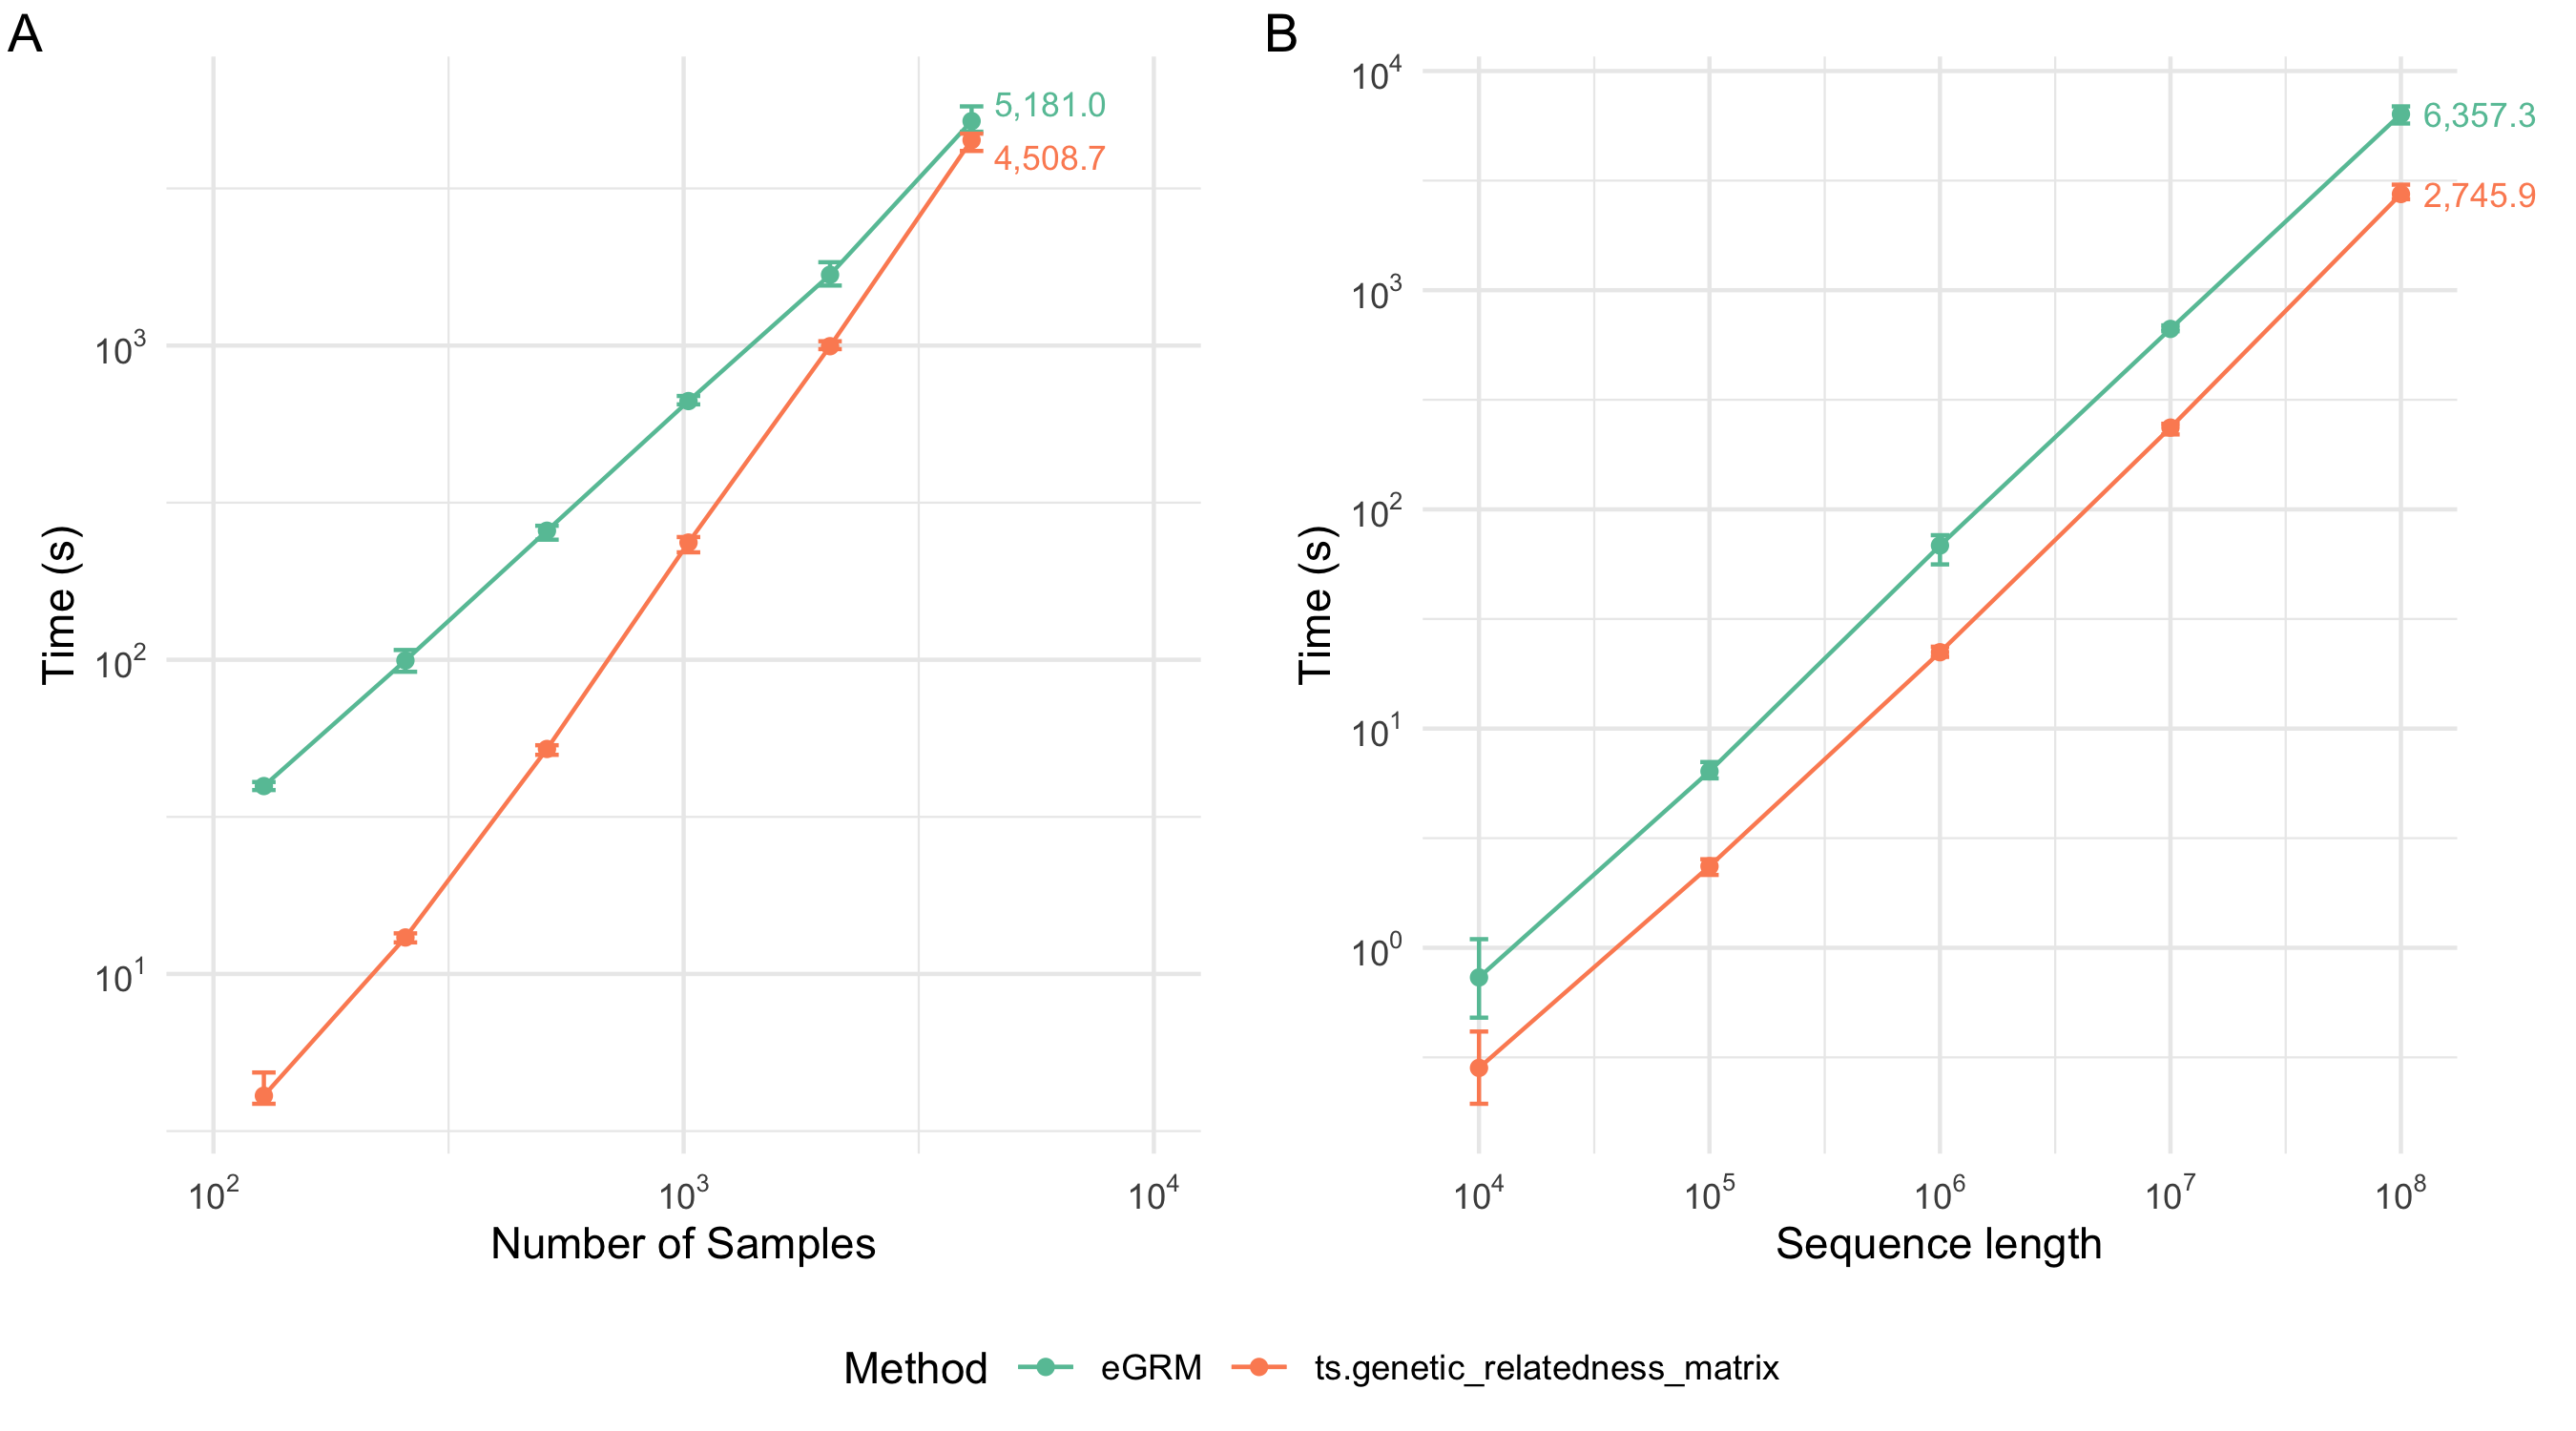
\includegraphics[width=\textwidth]{Figures/SIFig_benchmarking_plot.png}
    \label{fig:SI_benchmarking}
    \caption{Time efficiency of different implementations of branch GRM computation.
    Each dot corresponds to the average time taken across ten simulations with different random seeds.
    Error bars represent the range in time taken across the ten simulations.
    (A) Branch GRM computation with genome sequence length fixed at $10^{7}$ and varying the number of samples.
    (B) Branch GRM computation with number of sample nodes fixed at $2^{10}$ and varying genome sequence length.}
\end{figure}

\section{Proof of correctness of Algorithm V}\label{sec:proof-algv-correct}

Here we prove that when Algorithm V completes, $v(s)$ is equal to the
$s^{\text{th}}$ entry of $\mathbf{C}\mathbf{w}$, as defined
in~\eqref{eq:similar_ralph2020}.
In fact, after each step in the algorithm (i.e., after each addition or removal of an edge), 
it is true that for \textit{every} node $n$, the sum of everything above that node is equal to the weighted sum of covariances
for that node including everything up to that point in the genome.
In other words, for every $n$,
\begin{align} \label{eqn:matvec_consistent}
    S_T(n):=
    \sum_{r \ge_T n} v(r) + z(r)w(r) 
    = 
    \sum_{h:h \le k} (b_h-b_{h-1}) \sum_{r:n \le_{T_h} r} \ell_{T_h}(r) \sum_{t: t \le_{T_h} r} w_t
\end{align}
where $T$ is the current tree.
This statement reduces to our claim that the algorithm is correct because
the final tree is an ``empty'' tree with no edges,
so at the end of the algorithm, the left-hand side is simply $v(n)+z(n)$.
This is again $v(n)$ because $z(n)$ is zero due to $x(n)=b_K$.
The right-hand side is equal to equation 
(\ref{eq:similar_ralph2020}) when $n$ is a sample node.

Each time we add an edge with child $c$ and parent $p$ to the tree (step V2), 
we add the value of $w(n)$ to $p$ and all nodes above $p$ in the tree;
when removing edges we subtract (step V1).
Since $w(n)$ is initialized so that each sample $s$ carries $w_s$, this ensures that $w(n)= \sum_{s \le n} w_s$ at all times [as in \cite{kelleher2016efficient, ralph2020efficiently}].

We prove that equation  (\ref{eqn:matvec_consistent}) is always true by induction.
At the first (empty) tree, this is certainly true,
as both sides are equal to zero.
We now consider \textbf{Step V3}. 
Tree $T$ and the bookkeeping variables $v$, $w$ and $x$ are left constant.
Advancing the position from $k$ to $k+1$ only changes 
$z(s)=\ell_T(s) (b_k - x(s))$ to 
$z'(s)=\ell_{T'}(s) (b_{k+1} - x(s))$.
Therefore, the appended value to the left-hand side is
\begin{align}
    \sum_{r: n \le_T r}z'(r)w(r) - z(r)w(r) = (b_{k+1}-b_{k})
    \sum_{r: n \le_T r} \ell_T(r) w(r)
\end{align}
which is also equal to the added value to the right-hand side.
Note that this is the only step that changes the value of equation (\ref{eqn:matvec_consistent}).

\textbf{Step V1} and \textbf{V2} leave the value of both sides unchanged.
Without the loss of generality, we prove this for \textbf{V2}.
Suppose that we added edge $(c,p)$ where $c$ and $p$ are the child and the parent nodes of the edge, respectively.
We can divide the nodes of $\nodes$ into four categories as (1) the child node $c$, (2) nodes below $c$,  (3) the parent node $p$ and nodes above $p$, and (4) all other nodes. 
The insertion changes the values of the intermediate arrays to $v'$, $w'$, $z'$, and $x'$ following \textbf{V2}.
We denote the new tree resulting from the insertion as $T'$.

Observe that the difference in the left-hand side after $\mathbf{V2}$ is
\begin{align}
    \begin{aligned}
        &\sum_{r:n \le_{T'} r} v'(r) + z'(r)w'(r) 
        - \sum_{r:n \le_{T} r} v(r) + z(r)w(r)
        \\
        &= \sum_{r: n\le_{T'}r, n \nleq_T r } v'(r) + z'(r)w'(r) \\
        &+ \sum_{r: n \le_{T'} r, n\le_T r} v'(r)+z'(r)w'(r)-v(r)-z(r)w(r) \\
        &- \sum_{r: n \nleq_{T'} r, n\le_T r} v(r) + z(r)w(r) \\
        &=  \sum_{r: n\le_{T'}r, n \nleq_T r } v'(r) + z'(r)w'(r)\\
        &+ \sum_{r: n\le_T r} v'(r)+z'(r)w'(r)-v(r)-z(r)w(r)
    \end{aligned}
    \label{preserve_split}
\end{align}
for node $n$.
The last line follows from $\{r: n \le_T r \} \subset \{r: n\le_{T'} r\}$ because $T'$ has more edges than $T$.
Nodes in each category have distinct values for the former and the latter sum of this equation.

The set $\{r: n \le_{T'} r, n \nleq_T r\}$ of the first summation is
\begin{align}
    \begin{cases}
         \{r: p \le_{T'} r\} & \quad \text{$n$ in category (1) or (2)} \\
        \emptyset & \quad \text{$n$ in category (3) or (4)}
    \end{cases}
\end{align}
This is because $p$ and the nodes above $p$ are the nodes that were previously not ancestors in $T$, but became ancestors of $c$ and those below $c$ after the addition of the new edge.
The set is empty for the nodes in the third and the fourth category because their ancestor nodes are unchanged after edge insertion.
Therefore, the first summation is
\begin{align}
    \begin{cases}
        \sum_{r: p \le_{T'} r} v'(r) + z'(r)w'(r) & \quad \text{$n$ in category (1) or (2)} \\
        0 & \quad \text{$n$ in category (3) or (4)}
    \end{cases}
\end{align}

The summand of the second summation $v'(r) + z'(r) - v(r) - z(r)$ is
\begin{align}
    \begin{cases}
    v'(c) - v(c) & \quad \text{$r$ in category (1)} \\
    0 & \quad  \text{$r$ in category (2), (3), or (4)}
    \end{cases} 
\end{align}
For $r=c$ ($r$ is in the first category), it follows from $z(c)=0$ due to $\ell_T(c)=0$ and $z'(c)=0$ due to $x'(c)=b_k$.
All the bookkeeping values of the second and the fourth category is unchanged by \textbf{V2}, so the summand is trivially zero.
When $r=p$ ($r$ belongs to the third category), $v'(r) = v(r) + z(r)w(r)$  and $z'(r)=0$ by the operations $v(r) \pluseq z(r)w(r)$ and $x(r)=b_k$ by \textbf{V2}.
Hence, the second summation is
\begin{align}
    \begin{cases}
        v'(c) - v(c) & \quad \text{$n$ in category (1) or (2)} \\
        0 & \quad \text{$n$ in category (3) or (4)}
    \end{cases}
\end{align}
because the set $\{r: n \le_T r\}$ contains $c$ if and only if $n$ belongs to either the third or the fourth category.
An expression for $v'(c)-v(c)$ comes from the operation $v(c) \minuseq v(r)$ following $v(r) \pluseq z(r)w(r)$ of \textbf{V2}
\begin{align}
    v'(c) - v(c) = - \sum_{r: p \le_{T} r} v(r) + z(r)w(r)
\end{align}

Combining the aforementioned results, we see that equation (\ref{preserve_split}) is 
\begin{align}
    \begin{cases}
        \sum_{r: p \le_{T'} r} v'(r) + z'(r)w'(r) - \sum_{r: p \le_{T} r} v(r) + z(r)w(r) & \text{$n$ $\in$ (1) or (2)} \\
        0 & \text{$n$ $\in$ (3) or (4)}
    \end{cases} 
\end{align}
Both cases reduces to zero because the set of nodes ancestral to $p$ are the same in $T$ and $T'$ ($\{r: p \le_T r\}=\{r: p \le_{T'} r\}$), 
 and $v'(r) = v(r) + z(r)w(r)$ for these nodes due to \textbf{V2} and $z'(r)=0$. 

The right-hand side remains the same because the operation changes nothing in its expression:
it's the working sum until the previous local tree that it does not contain any of 
the components of the current tree that is being modified.
This completes the proof.

% --- Mixed ploidy -------------------------------------------------------

% \subsection{General ploidy}
% \peter{This section to be removed.}

% We now consider the covariance between $p$-ploid individuals,
% possibly different levels of ploidy.
% %
% Returning to the notation for trait in methods, suppose individual $i$ has
% ploidy $p_i$, then their trait genetic value is given by:
% %
% $$ 
% Z(i) = \sum_l \sum_{g=1}^{p_i} Z_{l,G_{i,l,g}}.
% $$
% %
% Let $n_g = \sum_{i=1}^{n_i} p_i$ be the total number of genome copies
% in the sample set of $n_i$ individuals.
% %
% The mean haploid value of the genome copies in individuals $1, \ldots, n_i$
% with genetic values $Z(1), \ldots, Z(n_i)$ is $\bar{Z}_g = (Z(1) + \cdots + Z(n_i))/n_g$.
% %
% If we center the value of each genome copy, then the centered trait value is given by:
% %
% \begin{align}
%   \tilde{Z}(i) &= \sum_{l} \sum_{g=1}^{p_i} \left( Z_{l,G_{i,l,g}} - \bar{Z}_g \right) \\
%                &= \sum_{l} \left( \sum_{g=1}^{p_i} Z_{l,G_{i,l,g}} - p_i\bar{Z}_g \right)
% \end{align}
% %
% Note that when $p_i = p$ for all $i$, then $n_g = n_i \times p$ and
% the above $\tilde{Z}(i)$ is equivalent to $Z(i) - \bar{Z}$.
% %
% This yields a general, including mixed, ploidy version of \eqref{eqn:trait_cov}:
% %
% \begin{align} \label{eqn:trait_cov_mixed}
%     \begin{split}
%         &\Cov\left[ \tilde{Z}(i), \tilde{Z}(j) \right]\\
%         &\qquad = \sum_l \Cov\left[ \left( \sum_{g=1}^{p_i} Z_{l,G_{i,l,g}} - p_i\bar{Z}_g \right)
%                                     \left( \sum_{g=1}^{p_j} Z_{l,G_{j,l,g}} - p_j\bar{Z}_g \right) \right]\\
%         &\qquad = \sigma^2 / 2 \sum_l \sum_a
%                                \left(n(i,l,a) - p_i\bar{n}(l,a)\right)
%                                \left(n(j,l,a) - p_j\bar{n}(l,a)\right).
%     \end{split}
% \end{align}
% %
% This general ploidy formulation opens the opportunity to compute relatedness
% between individuals of any ploidy as well as between sets of individuals
% grouped in some way, say, by population.
% %
% These sets will often vary in size, hence the need for the general ploidy formulation.

% --- Computing with tree statistics -------------------------------------

% \subsection{Computing with tree statistics}
% \label{sec:treestats}

% In summary,
% let $n_g = \sum_{i=1}^{n_i} p_i$ and
% let $\bar{x} = \frac{1}{n_g}\sum_{g=1}^{n_g} x_g$.
% %
% Let
% %
% \begin{align}
%     f_{i,j}(x_1, \ldots, x_{n_i})
%     &= \frac{1}{2} \left(x_i - p_i \bar{x} \right)
%                    \left(x_j - p_j \bar{x} \right)
% \end{align}
% %
% and for each sample node $g$ and individual $i$ let
% $w_{g,i} = 1$ if $g$ is a genome copy of individual $i$, and
% $w_{g,i} = 0$ otherwise.
% %
% Let $T$ be the unpolarised, not span normalised,
% site statistic with the summary function $f_{i,j}$ and a matrix of weights $\mathbf{W}$.
% %
% Then, $T$ is exactly equation \eqref{eqn:trait_cov_mixed} and
% the following equivalences hold:
% %
% \begin{itemize}
%     \item 
%         $T$ is equal to $\Cov\left[Z(i) - \bar{Z}, Z(j) - \bar{Z}\right]$,
%         as in equation \eqref{eqn:trait_cov}.
        
%     \item 
%         If all sites are bi-allelic,
%         and $n_l$ is the number of loci,
%         then $T/n_l = C_{i,j}$,
%         as in equation \eqref{eqn:grm}.
        
%     \item
%         $T$ has the following interpretation:
%         let $m(i ,j)$ denote the total number of pairwise allele matches
%         between the genomes of individual $i$ and of individual $j$,
%         and let $U$ and $V$ be independently chosen individuals from the set of individuals.
%         Then $T$ is the number of pairwise allele matches between $i$ and $j$
%         relative to the rest of the samples:
%         $T = \E[m(i,j) - m(i,U) - m(j,V) + m(U,V)]$,
%         as in equation \eqref{eqn:relative_allele_matches}.
        
% \end{itemize}

% To obtain covariances of the non-centered values
% (i.e., for $Z(i)$ not $Z(i) - \bar Z$),
% one uses
% \begin{align*}
%     f_{i,j}(x_1, \ldots, x_{n_i})
%     = x_i x_j ,
% \end{align*}
% with a \emph{polarised} statistic.

% --- Weighted sums ------------------------------------------------------

% TODO: GG continue parsing/polishing here (see notation.text!)
% N_p --> n_g
% N --> n_i
% I --> i
% J --> i
% i --> ???
% j --> ???

% \subsection{Weighted sums}

% \todo[inline]{TODO: $Z(\mathbf{W})_i$ notation is confusing}

% Let $\mathbf{W}$ be a $n_g \times n_i$ matrix of weights,
% where $n_g$ is the number of genome copies and $n_i$ is number of individuals,
% and let $Z(\mathbf{W})_k = \sum_i \mathbf{W}_{k,i} Z(i)$.
% %
% \todo[inline]{TODO: this $_k$ is confusing because the sum is supposed to go over
% individuals (denoted with $i$) to get $k-$th $Z(\mathbf{W})_k$,
% but unclear what is this quantity!
% Below we have $Z(\mathbf{W})_I$ indicating that $_k$ is indexing individuals,
% but above definition suggests it's sum over individual's values for $k-$th genome?}
% %
% Let $\bar{Z}$ be defined appropriately. (???)
% %
% Let $f_{i,j}$ be as above, and let the weights be given by $\mathbf{W}$.
% %
% Then
% $$
%     T = \Cov\left[Z(\mathbf{W})_I - \bar{Z}, Z(\mathbf{W})_J - \bar{Z}\right] .
% $$
% \todo{TODO: Change $I$ and $J$ to $i$ and $j$ once above confusion is cleared.}
% %
% So, for instance, suppose we want to compute
% $\Cov\left[Z(i), \sum_? w_? Z(?)\right]$, for each $i$.
% %
% Then we would use a matrix of weights $\mathbf{W}$ as above,
% with an extra column for $w$,
% and the summary function
% $(f_{1,n_i+1}, f_{2,n_i+1}, f_{3,n_i+1}, \ldots, f_{n_i, n_i+1})$.
% %
% And figure out what happens with $\bar{Z}$. (???)

% --- Matrix-vector multiplications --------------------------------------

% \subsection{Matrix-vector multiplications}

% In terms of a GP kernel matrix $\mathbf{K}$ on \textit{individuals}
% (rather than haplotypes), we have:
% %
% $$
%     \mathbf{K}_{i,j} = \Cov\left[Z(i) - \bar{Z}, Z(j) - \bar{Z}\right].
% $$
% %
% Or, writing $\tilde{\mathbf{Z}} = (Z(1) - \bar{Z}, \dots, Z(n_i) - \bar{Z})$,
% then $\mathbf{K} = \Var\left[\tilde{\mathbf{Z}}\right] \equiv \Cov\left[\tilde{\mathbf{Z}}, \tilde{\mathbf{Z}}\right]$.

% Suppose we want to evaluate $\mathbf{Kb}$ for a vector $\mathbf{b}$.
% %
% We have:
% %
% $$ \mathbf{Kb} = \Cov\left[\tilde{\mathbf{Z}}, \mathbf{b}^T\tilde{\mathbf{Z}}\right] $$
% %
% So the $i^{th}$ component of $\mathbf{Kb}$ is:
% %
% \begin{align}
%     (\mathbf{Kb})_i &= \Cov\left[ Z(i) - \bar{Z}, ~\sum_{j=1}^{n_i} b_j \left(Z(j) - \bar{Z} \right) \right] \\
%                     &= \Cov\left[ Z(i) - \bar{Z}, ~\sum_{j=1}^{n_i} b_j Z(j) - \sum_{j=1}^{n_i} b_j \bar{Z} \right]
% \end{align}
% %
% Factoring out $\sum{j=1}^{n_i} b_j = B$,
% $$
%     (\mathbf{Kb})_i = B \times \Cov\left[ Z(i) - \bar{Z}, ~\sum_{j=1}^{n_i} (b_j/B) Z(j) - \bar{Z} \right],
% $$
% so $\bar{Z}$ doesn't need changing!(?)

% We also have
% $$
%     (\mathbf{Kb})_i = \sum_{j=1}^{n_i} b_j \Cov\left[ Z(i) - \bar{Z}, ~Z(j) - \bar{Z} \right] 
% $$

% Using equation \eqref{eqn:trait_cov_mixed}:
% %
% % TODO: polish
% \begin{align}
%     (\mathbf{Kb})_i
%         &= \sigma^2 / 2 \sum_{j=1}^N b_j \sum_k \sum_a
%             \left(n_k(I,a) - p_I\bar{n}(k,a)\right) \left( n_k(j, a) - p_j\bar{n}(k,a)\right) \\
%         &= \sigma^2 / 2 \sum_k \sum_a
%             \left(n_k(I,a) - p_I\bar{n}(k,a)\right) \sum_{j=1}^N b_j  \left( n_k(j, a) - p_j\bar{n}(k,a)\right) \\
%         &= \sigma^2 / 2 \sum_k \sum_a
%             \left(n_k(I,a) - p_I\bar{n}(k,a)\right) \left(\sum_{j=1}^N b_j n_k(j, a) - \bar{n}(k,a)\sum_{j=1}^N b_jp_j \right)
% \end{align}

% So, given the weight matrix above, the summary function we want is 
% %
% $$\begin{aligned}
%  f_{i,j}(x_1, \ldots, x_{n_i})
%  &= \frac{1}{2} \left(x_i - \bar{x}\sum_? W_{?,i} \right)
%                 \left(x_j - \bar{x}\sum_? W_{?,j} \right).
% \end{aligned}$$
% %
% This is equivalent to the previous summary function, since $p_i = \sum_? \mathbf{W}_{?,i}$.

% --- Kinship matrices ----------------------------------------------------

% \subsection{Kinship matrices}

% \todo[inline]{Most of this is now in methods.tex! Should we remove this sub-section?}

% One definition of the kinship matrix between individuals $i$ and $j$ is
% that $K_{i,j}$ is equal to
% ``the probability of a match between alleles drawn at random from each of them'',
% averaged over sites and with the alleles drawn with replacement if $i=j$
% (Speed \& Balding, definition of $K_{as}$).
% %
% Note that the probability of a match between two randomly chosen alleles
% is equal to the number of pairwise matches divided by $p^2$,
% where $p$ is the ploidy.
% %
% To get $K_{as}(i,j)$,
% we would take the summary function $x_i x_j$ and divide by $p^2 n_?$.
% %
% Another definition of Speed \& Balding is $K_{c0}$,
% and is equal to equation \eqref{eqn:grm}.

% --- Polarisation -------------------------------------------------------

% \subsection{Polarisation}

% Let $S'$ denote the \emph{polarised} site statistic with
% summary function $f_{i,j}$ and weights $w$.
% %
% This is simply equation \eqref{eqn:compute_C}
% but where the sum is over all \emph{non-ancestral} alleles,
% and so is equal to:
% %
% \begin{itemize}
%     \item
%         The number of pairwise matches of \emph{non-ancestral} alleles between $i$ and $j$
%         relative to random individuals, as above.
%     \item
%         $\Cov[Z(i) - \bar{Z}, Z(j) - \bar{Z}]$
%         instead the ancestral allele has zero effect and
%         derived alleles have variance $\sigma^2 / 2$.
% \end{itemize} 

% Note in particular that if all sites are bi-allelic,
% then the two components of \eqref{eqn:trait_cov} obtained by each of the two alleles are equal
% (since $(a-c)(b-d) = ((n-a)-(n-c))((n-b)-(n-d))$),
% and so the polarised statistic is just equal to one-half of the unpolarised statistic.
